\section{实验一:Xv6 and Unix utilities}\label{sec:Xv6 and Unix utilities}

使用系统调用编写一些实用程序。

\subsection{实验目的}

\begin{enumerate}
	\item 初步掌握 xv6 这一操作系统内核和用户。
	\item 了解系统调用。
	\item 了解父子进程,以及 \texttt{fork()}函数创建父子进程的方法。
	\item 掌握素数筛,以及利用管道编写素数筛的方法。
	\item 完成 \texttt{find} 和 \texttt{xargs} 程序的编写。
\end{enumerate}

\subsection{实验内容}

\begin{enumerate}
	\item 运行xv6
	\item 为 xv6 实现 UNIX 程序 \texttt{sleep}:sleep 应该暂停一段用户所指定的时间。
	\item 编写一个程序,使用 UNIX 系统调用在两个进程之间通过一对管道“乒乓” 一个字节,每个管道一个。
	\item 使用管道编写并发版本的主筛。
	\item 编写一个简单版本的 UNIX 查找程序:查找具有特定名称的目录树中的所有文件。
	\item 编写一个简单版本的 UNIX xargs 程序:从标准输入中读取行并为每一行运行一个命令,将该行作为命令的参数提供。
\end{enumerate}

\subsection{实验准备}

该实验是为了让学习者熟悉 xv6 及其系统调用,没有前置条件。

\subsection{实验步骤}

\subsubsection{运行xv6}

\begin{enumerate}
	\item 在命令行中输入 git clone git://g.csail.mit.edu/xv6-labs-2021 克隆项目
	\item 进入项目目录,输入 git checkout 切换到util分支,如\cref{fig:change_to_util} 所示。
	\item 安装需要的依赖项。
	\item 使用 make qemu 指令运行,如\cref{fig:make_qemu} 所示。
	\item 使用 ls 命令查看文件,如\cref{fig:ls} 所示。
\end{enumerate}

\begin{figure}[!htb]
	\centering
	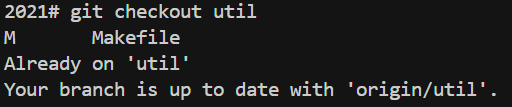
\includegraphics[width=0.5\textwidth]{change_to_util}
	\caption{切换到util分支}
	\label{fig:change_to_util}
\end{figure}

\begin{figure}[!htb]
	\centering
	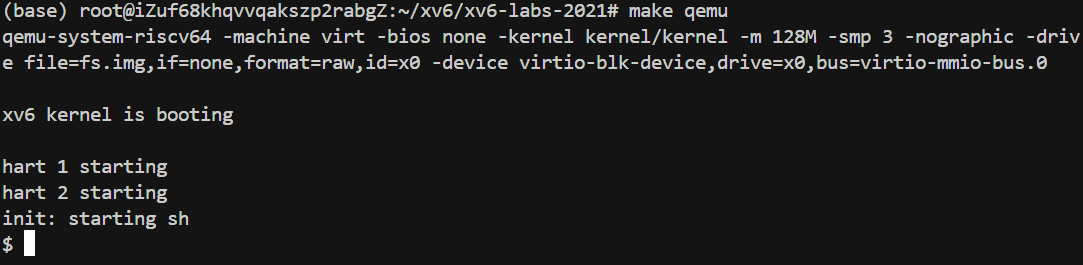
\includegraphics[width=1\textwidth]{make_qemu}
	\caption{使用 make qemu 指令运行}
	\label{fig:make_qemu}
\end{figure}

\begin{figure}[!htb]
	\centering
	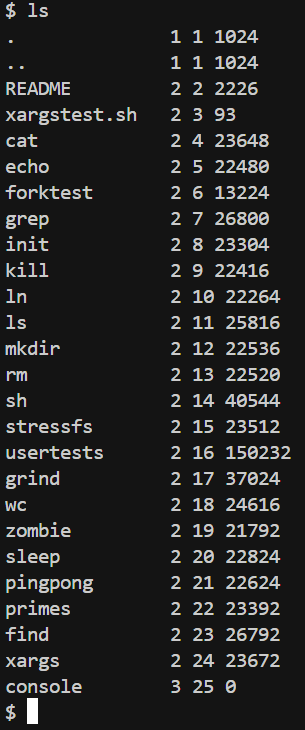
\includegraphics[width=0.25\textwidth]{ls}
	\caption{使用 ls 命令查看文件}
	\label{fig:ls}
\end{figure}

\subsubsection{实现sleep}

实现步骤:
\begin{enumerate}
	\item 查看系统调用函数,学习如何获取传递给程序的命令行参数,如\cref{lst:echo} 所示。
	\item 获取下标为1的所给参数,将其转化为整数类型,并调用系统函数,如\cref{lst:sleep} 所示。
	\item 在Makefile文件中添加该方法
	\item 测试sleep方法,结果如\cref{fig:test_sleep} 所示。
\end{enumerate}

\begin{listing}[!htb]
	\begin{minted}{c}
int
main(int argc, char *argv[])
{
    int i;

    for(i = 1; i < argc; i++){
        write(1, argv[i], strlen(argv[i]));
        if(i + 1 < argc){
            write(1, " ", 1);
        } else {
            write(1, "\n", 1);
        }
    }
    exit(0);
}
	\end{minted}
	\caption{xv6的echo方法实现}\label{lst:echo}
\end{listing}

\begin{listing}[!htb]
	\begin{minted}{c}
int
main(int argc, char *argv[]){
    if(argc<2){
        printf("Error:No argument\n");
    }
    else if(argc>2){
        printf("Error:Too much argument\n");
    }
    else{
        int tag = 1;
        char *p = argv[1];
        while(*p){
        if(*p<'0'||*p>'9'){
            tag=0;
            break;
        }
        p++;
    }
    if(tag){
        sleep(atoi(argv[1]));
    }
    else{
        printf("Error:Illegal argument\n");
        }
    }
    exit(0);
}
	\end{minted}
	\caption{sleep方法的实现}\label{lst:sleep}
\end{listing}

\begin{figure}[!htb]
	\centering
	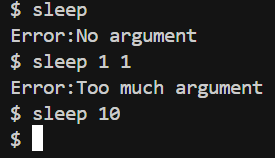
\includegraphics[width=0.4\textwidth]{test_sleep}
	\caption{测试sleep方法}
	\label{fig:test_sleep}
\end{figure}

\subsubsection{实现pingpong}

从概念上讲,管道是两个进程之间的连接,使得一个进程的标准输出成为另一个进程的标准输入。在 UNIX 操作系统中,管道用于相关进程之间的通信(进程间通信)。
关于管道的详细说明:
\begin{enumerate}
	\item 管道是单向通信,也就是说,我们可以使用管道,一个进程向管道写入数据,另一个进程从管道读取数据。它打开一个管道,该管道是主内存中的一块区域,被视为“虚拟文件”。
	\item 创建进程及其所有子进程都可以使用该管道进行读写操作。一个进程可以向这个“虚拟文件”或管道写入数据,而另一个相关进程则可以从中读取数据。
	\item 如果某个进程在将某些内容写入管道之前尝试读取,则该进程将被暂停,直到写入某些内容为止。
	\item 管道系统调用在进程的打开文件表中找到前两个可用位置,并将它们分配给管道的读写端。
\end{enumerate}

\begin{figure}[!htb]
	\begin{minipage}{0.4\textwidth}
		\centering
		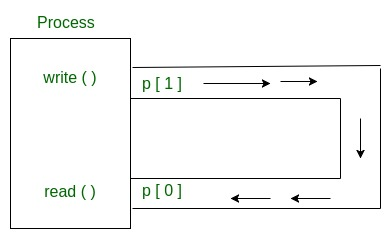
\includegraphics[width=\textwidth]{pipe}
		\caption{管道示意图}
		\label{fig:pipe}
	\end{minipage}\hfill
	\begin{minipage}{0.4\textwidth}
		\centering
		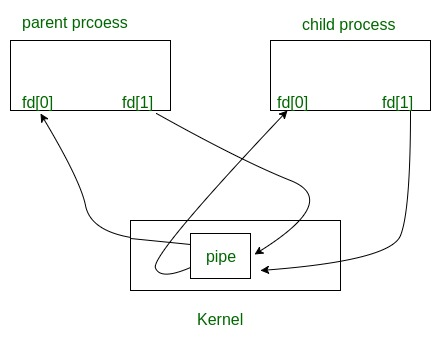
\includegraphics[width=\textwidth]{sharing_pipe}
		\caption{父子进程共用管道}
		\label{fig:sharing_pipe}
	\end{minipage}
\end{figure}

实现步骤:
\begin{enumerate}
	\item 创建管道。
	\item 创建缓冲区,用于存储所需要传送的消息。同时,借助 \texttt{fork()}创建子进程,通过返回值来判断当前是父进程还是子进程,返回值大于0是父进程,等于0是子进程。
	\item 在Makefile文件中添加该方法
	\item 测试pingpong方法,结果如\cref{fig:pingpong} 所示。
\end{enumerate}

\begin{listing}[!htb]
	\begin{minted}{c}
int
main(){
    int p[2];
    pipe(p); 
    int pid = fork();
    if(pid == 0){ // 子进程
        close(p[1]); // 关闭写端
        read(p[0],&pid,4);
        printf("\%d: received ping\n",getpid());
        close(p[0]); // 关闭读端
        exit(0); // 释放子进程资源
    }
    else{
        close(p[0]);
        write(p[1],&pid,4);
        close(p[1]);
        wait(0); // 等待子进程结束后再输出
        printf("\%d: received pong\n",getpid());
    }
    exit(0);
}
	\end{minted}
	\caption{pingpong方法的实现}\label{lst:test_pingpong}
\end{listing}

\begin{figure}[!htb]
	\centering
	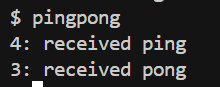
\includegraphics[width=0.4\textwidth]{test_pingpong}
	\caption{测试pingpong方法}
	\label{fig:test_pingpong}
\end{figure}

\subsubsection{实现primes}

在本题中,素数筛的原理是:生成进程可以将数字 2、3、4、...、1000 输入到管道的左端:管道中的第一个进程消除 2 的倍数,第二个进程消除 3 的倍数,第三个进程消除 5 的倍数,依此类推。如\cref{fig:sieve} 所示。

\begin{figure}[!htb]
	\centering
	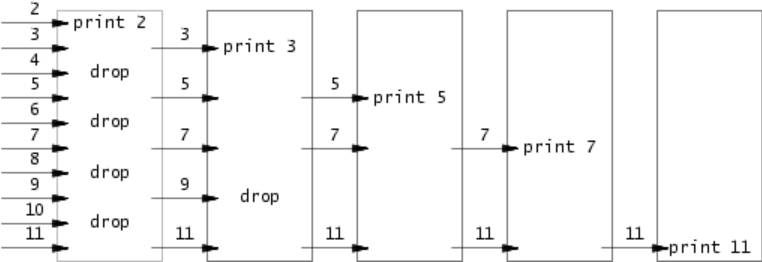
\includegraphics[width=0.6\textwidth]{sieve}
	\caption{素数筛示意图}
	\label{fig:sieve}
\end{figure}

实现步骤:
\begin{enumerate}
	\item 借助父子进程的并发性,同时利用上一小问中所学习到的管道通信机制来传输消息。
	\item 注意当不需要的时候需要及时释放资源,否则将会资源不足。
	\item 在Makefile文件中添加该方法。
	\item 测试primes方法,结果如\cref{fig:test_primes} 所示。
\end{enumerate}

\begin{listing}[!htb]
	\begin{minted}{c}
void get_primes(int p1[2]){
    close(p1[1]);
    int n; // 当前数字
    int tag = read(p1[0],&n,4);
    if(tag == 0){
        close(p1[0]);
        exit(0);
    }
    printf("prime \%d\n",n)
    int p2[2];
    pipe(p2);
    int pid = fork();
    if(pid == 0){
        get_primes(p2);
    }
    else{
        int m;
        close(p2[0]);
        while(read(p1[0],&m,4)){
            if(m \% n!=0){
                write(p2[1],&m,4);           
            }
        }
        close(p2[1]);
        wait(0);
    }
}

int
main(){
    int p[2];
    pipe(p);
    for(int i = 2;i<35;i++){
        write(p[1],&i,4);
    }
    get_primes(p);
    close(p[1]);
    exit(0);
}
	\end{minted}
	\caption{primes方法的实现}\label{lst:primes}
\end{listing}

\begin{figure}[!htb]
	\centering
	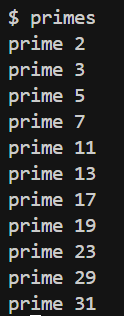
\includegraphics[width=0.2\textwidth]{test_primes}
	\caption{测试primes方法}
	\label{fig:test_primes}
\end{figure}

\subsubsection{实现find}

实现步骤:
\begin{enumerate}
	\item 查看 \texttt{user/ls.c} 学习如何读取目录。
	\item 采用深度优先的方法进行递归,需要注意避免递归"."和"..",防止无限递归。
	\item 在 Makefile 文件中添加该方法。
	\item 测试 \texttt{find} 方法,结果如\cref{fig:test_find} 所示。
\end{enumerate}

\begin{listing}[!htb]
	\begin{minted}{c}
char*
fmtname(char *path)
{
    static char buf[DIRSIZ+1];
    char *p;
    // Find first character after last slash.
    for(p=path+strlen(path); p >= path && *p != '/'; p--)
    ;
    p++;
    // Return blank-padded name.
    if(strlen(p) >= DIRSIZ)
    return p;
    memmove(buf, p, strlen(p));
    memset(buf+strlen(p), 0, DIRSIZ-strlen(p));
    return buf;
}

int recurse(char *path){
    char *p = fmtname(path);
    if((p[0] == '.' && p[1] == 0) || (p[0] == '.' && p[1]=='.'&&p[2]==0)){
        return 0;
    }
    return 1;
}
	\end{minted}
	\caption{find方法的实现(1)}\label{lst:find1}
\end{listing}

\begin{listing}[!htb]
	\begin{minted}{c}
void
find(char *path,char *target)
{
    char buf[512], *p;
    int fd;
    struct dirent de;
    struct stat st;

    if((fd = open(path, 0)) < 0){
        fprintf(2, "ls: cannot open \%s\n", path);
        return;
    }
    if(fstat(fd, &st) < 0){
        fprintf(2, "ls: cannot stat \%s\n", path);
        close(fd);    
        return;
    }
    // 比较
    if(strcmp(fmtname(path),target)==0){
        printf("\%s\n",path);
    }
    switch(st.type){
        case T_FILE:
        break;
        case T_DIR:
        if(strlen(path) + 1 + DIRSIZ + 1 > sizeof buf){
            printf("ls: path too long\n");    
            break;
        }
        strcpy(buf, path);
        p = buf+strlen(buf);
        *p++ = '/';
        while(read(fd, &de, sizeof(de)) == sizeof(de)){
            if(de.inum == 0)
            continue;
            memmove(p, de.name, DIRSIZ);
            p[DIRSIZ] = 0;
            
            if(stat(buf, &st) < 0){
                printf("ls: cannot stat %s\n", buf);
                continue;
            }
            // 判断递归
            if(recurse(buf) == 1){
                find (buf,target);
            }
        }
        break;
    }
    close(fd);
}
	\end{minted}
	\caption{find方法的实现(2)}\label{lst:find2}
\end{listing}

\begin{listing}[!htb]
	\begin{minted}{c}
int
main(int argc, char *argv[])
{
    if(argc==1){
        printf("Error:No argument\n");
        exit(0);
    }
    else if(argc == 2){
        find(".",argv[1]);
        exit(0);
    }
    else if(argc == 3){
        find(argv[1],argv[2]);
        exit(0);
    }
    else{
        printf("Error:Too much argument\n");
        exit(0);
    }
    exit(0);
}
	\end{minted}
	\caption{find方法的实现(3)}\label{lst:find3}
\end{listing}

\begin{figure}[!htb]
	\centering
	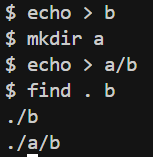
\includegraphics[width=0.25\textwidth]{test_find}
	\caption{测试find方法}
	\label{fig:test_find}
\end{figure}

\subsubsection{实现xargs}

\texttt{xargs} 是一个 Unix 命令,可用于从标准输入构建和执行命令。其作用是将标准输入(stdin)中的内容,转换为命令行参数,传递给指定的命令执行。

\texttt{exec} 命令是一个强大的 Shell 内置命令,用于将当前 Shell 进程替换为新的命令进程。与创建新进程的典型命令不同, \texttt{exec} 命令会转换现有进程,直接影响脚本的效率和行为。\texttt{exec} 会使用指定的命令覆盖当前 Shell 会话,而不会创建新的进程。这一独特属性使得 \texttt{exec} 在修改 Shell 环境或执行注重性能的命令时特别有用,因为它避免了创建新进程的开销。

实现步骤:
\begin{enumerate}
	\item 学习 \texttt{xargs} 和 \texttt{exec} 命令的作用及用法。
	\item 需要解决的主要问题是对字符串进行处理。其中,'|' 之前的结果会在缓冲流中。需要通过读取缓冲流并且分解字符串,类似于 python 中的 split 函数。
	\item 在Makefile文件中添加该方法。
	\item 测试 \texttt{xargs} 方法,结果如\cref{fig:test_xargs} 所示。
\end{enumerate}

\begin{listing}[!htb]
	\begin{minted}{c}
int
main(int argc,char *argv[]){
    sleep(10);
    
    // 获取前一个命令的标准化输出
    char buf[BUFFER_SIZE];
    read(0,buf,BUFFER_SIZE);

    // 获取自己的命令行参数
    char *xargv[MAXARG];
    int xargc = 0;

    for(int i=1;i<argc;i++){
        xargv[xargc] = argv[i];
        xargc++;
    }

    char *p = buf;
    for(int i = 0;i < BUFFER_SIZE;i++){
        if(buf[i] == '\n'){
            int pid = fork();
            if(pid > 0){
                p = &buf[i+1];
                wait(0);
            }
            else{
                // 使用 exec去执行命令
                buf[i] = 0;
                xargv[xargc] = p;
                xargc++;
                xargv[xargc] = 0; // 对于exec,xargv最后一个元素必须是0
                xargc++;

                exec(xargv[0],xargv);
                exit(0);
            }
        }
    }

    exit(0);
}
	\end{minted}
	\caption{xargs方法的实现}\label{lst:xargs}
\end{listing}

\begin{figure}[!htb]
	\centering
	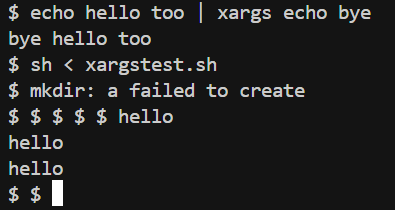
\includegraphics[width=0.5\textwidth]{test_xargs}
	\caption{测试xargs方法}
	\label{fig:test_xargs}
\end{figure}

\subsubsection{综合测试}

在xv6-labs-2021目录下创建一个time.txt文件,记录我完成该lab花费的时间,使用 \texttt{make grade} 对lab1进行综合测试,测试通过。

\begin{figure}[!htb]
	\centering
	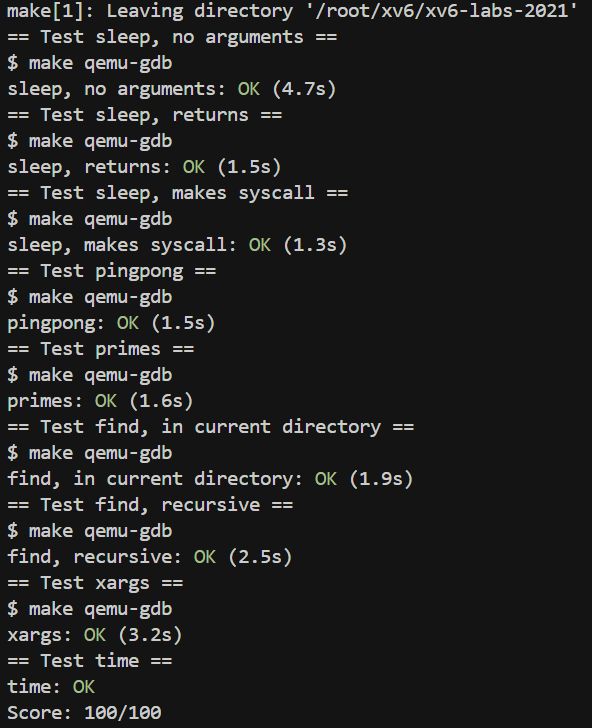
\includegraphics[width=0.5\textwidth]{test_lab1}
	\caption{lab1综合测试}
	\label{fig:test_lab1}
\end{figure}

\subsection{实验小结}

通过本实验,我初步了解了 xv6 这一操作系统内核,同时也了解了 qemu 模拟器的使用方法。
在完成实验的过程中,我遇到了比较多的困难,包括不知道管道如何创建、创建完成后如何关闭、素数筛到底是什么等等。但是通过和同学交流以及利用网络资源,我成功的解决了这些问题。
此外,我还初步了解到了系统调用接口,并且直到了操作系统内核和用户的一个区别。




